% Main Thesis File: This is the main file and it connects all the different parts of the thesis and compiles it into a single outcome file.

\documentclass[onecolumn, 12 pt, doublespace, fullpage, letterpaper]{report}
\renewcommand{\baselinestretch}{1.75}

% Packages
\usepackage{amssymb}
\usepackage{textcomp}
\usepackage{graphicx}
\usepackage{graphics}
\usepackage{epsfig}
\usepackage{epstopdf}
\usepackage{float}
\usepackage{color}
\usepackage[cmex10]{amsmath}
\usepackage{latexsym,amsfonts}
\usepackage{amsthm}
\usepackage{url}
\usepackage{longtable}
\usepackage[figuresright]{rotating}
\usepackage{listings}

\usepackage{fancyhdr}       
\pagestyle{fancy} 
\fancyhead{} \fancyfoot{} 
\fancyhead[CO,CE]{\thepage}      
\renewcommand{\headrulewidth}{0pt}


\usepackage{setspace}
\usepackage{subfigure}

% ### Nomenclature, List of Abbreviations and List of Symbols 
   \usepackage{ifthen,xkeyval,xfor,amsgen}
   \usepackage[acronym,toc]{glossaries}
   \newglossary[slg]{symbols}{syi}{sbl}{List of Symbols}
   \makeglossaries
   
   
% #### Symbols ####
\newglossaryentry{symb:Pi}{
name=$\pi$, type=symbols,
description=A mathematical constant whose value is the ratio of any circle's circumference to its diameter,
sort=symbolpi
}

\newglossaryentry{symb:Phi}{
name=$\varphi$, type=symbols,
description=An angle,
sort=symbolphi
}

\newglossaryentry{symb:Lambda}{
name=$\lambda$, type=symbols,
description={Lambda indicates usually an eigenvalue in linear algebra},
sort=symbollambda
}

% #### Abbreviations ####
\newacronym{toc}{ToC}{Table of Contents}
\newacronym{los}{LoS}{List of Symbols}
\newacronym{loa}{LoA}{List of Abbreviations}
\newacronym{phd}{PhD}{Doctoral}
\newacronym{MS}{MS}{Masters}
\newacronym{M$}{MS}{Microsoft}
\newacronym{CD}{CD}{Compact Disc}
\newacronym{kaust}{KAUST}{King Abdullah University of Science and Technology}

%An acronym with a glossary entry
\newacronym{AD}{AD}{Active Directory\protect\glsadd{glos:AD}}



% #### Nomenclature terms ####
\newglossaryentry{glos:AD}{
name=Active Directory,
description={Active Directory is the directory service for Windows based networks, that allows central organization and administration of any network resource. It allows a single-sign-on concept independent from network topologies or network protocols. As a prerequisite you need a Windows Server acting as Domain Controller. This computer stores all necessary data, e.g.~usernames and corresponding passwords}
}

\newglossaryentry{glos:RespF}{name=response file, description={A file 
that allows unattended software installation}}


   % Run the following three lines in the command line to get the lists
%makeindex -s Thesis.ist -t Thesis.alg -o Thesis.acr Thesis.acn
%makeindex -s Thesis.ist -t Thesis.slg -o Thesis.syi Thesis.sbl
%makeindex -s Thesis.ist -t Thesis.glg -o Thesis.gls Thesis.glo

% ### End of addition

\usepackage{hyperref} 


% Modified commands
\newcommand{\Tab}{\hspace{2ex}}
\usepackage[lmargin=1.5in, rmargin=1in, vmargin=1in]{geometry}
\newcommand{\mathsym}[1]{{}}
\newcommand{\unicode}[1]{{}}
\renewcommand{\thechapter}{\Roman{chapter}}
\renewcommand\bibname{\centering BIBLIOGRAPHY}



\begin{document}

\vspace{2pt}
\thispagestyle{empty}
\addvspace{10mm}

\begin{center}
{\bf\Large Your Thesis Title}\vfill
{\Large Thesis by}\\
{\bf\Large Your Full Name, Your Latest Earned Degree Title}\vfill
{\Large Submitted in Partial Fulfillment of the Requirements for the degree of}\\
{\bf\Large Masters of Science/Doctor of Philosophy}\vfill
{King Abdullah University of Science and Technology}\\\vspace{2pt}
{Your Division Name}\\\vspace{2pt}
{Your Program Name}\vfill
%\maketitle
{Thuwal, Makkah Province, Kingdom of Saudi Arabia}\\
{Full Month, Year}\vfill

\end{center}

\newpage
\noindent{The undersigned approve the thesis of Your Full Name}\vfill

\begin{flushleft}
\rule{15em}{1pt} \hfill \rule{10em}{1pt} \hfill \rule{6em}{1pt} \\\vspace{-5pt}
\makebox[15em][l]{Dr. Committee Member 1 Name} \hfill \makebox[10em][l]{Signature} \hfill \makebox[6em][l]{Date}\\\vspace{-5pt}
\makebox[15em][l]{Committee Member}\\\vspace{5em}

\rule{15em}{1pt} \hfill \rule{10em}{1pt} \hfill \rule{6em}{1pt} \\\vspace{-5pt}
\makebox[15em][l]{Dr. Committee Member 2 Name} \hfill \makebox[10em][l]{Signature} \hfill \makebox[6em][l]{Date}\\\vspace{-5pt}
\makebox[15em][l]{Committee Member}\\\vspace{5em}

\rule{15em}{1pt} \hfill \rule{10em}{1pt} \hfill \rule{6em}{1pt} \\\vspace{-5pt}
\makebox[15em][l]{Dr. Advisor's Name} \hfill \makebox[10em][l]{Signature} \hfill \makebox[6em][l]{Date}\\\vspace{-5pt}
\makebox[15em][l]{Committee Chair(Thesis Supervisor)}
\end{flushleft}\vfill

\begin{center}
{King Abdullah University of Science and Technology}\\
{Year}
\end{center}

\newpage
\vspace*{\fill}
\begin{center}
{Copyright \copyright Year}\\
{Your Full Name}\\
{All Rights Reserved}
\end{center}

% Abstract

\pdfbookmark[1]{Abstract}{Abstract} % Bookmark name visible in a PDF viewer

\begingroup
\let\clearpage\relax
\let\cleardoublepage\relax
\let\cleardoublepage\relax

\chapter*{Abstract} % Abstract name

Short summary of the contents\dots

\endgroup			

\vfill


% Acknowledgments File

\chapter*{Acknowledgments}

%\addcontentsline{toc}{chapter}{Acknowledgments} % Commented out by Christos: section precedes TOC

I would like to sincerely thank my supervisor Dr. Advisor's Name for his continuous guidance and encouragement throughout the course of this work. His enthusiasm and valuable feedback for research made my study very enjoyable and exciting and ultimately fruitful with rich experience. I would also like to thank him for providing me with an amazing research environment.

I thank my parents for their continuous encouragement and my siblings for bearing with me for my negligence towards them during this journey and their deep moral support at all times.

Lastly, I would like to thank the people at KAUST, Thuwal, Makkah Province, Saudi Arabia for providing support and resources for this research work.

% Copyright 2010 Imran Shafique Ansari
% Contact Email: imran.ansari@kaust.edu.sa
% Contact Number: +966 59 897 1005


\renewcommand{\contentsname}{TABLE OF CONTENTS}
\tableofcontents
\cleardoublepage

\printglossary[type=\acronymtype,style=long3col, title=List of Abbreviations, toctitle=List of Abbreviations, nonumberlist=true] 
\printglossary[type=symbols,style=long3col, nonumberlist=true] 

\renewcommand*\listfigurename{List of Illustrations} 
\addcontentsline{toc}{chapter}{\listfigurename} 
\listoffigures

\cleardoublepage
\addcontentsline{toc}{chapter}{\listtablename}
\listoftables

% \printglossary[style=altlist,title=Nomenclature, toctitle=Nomenclature, nonumberlist=true] 


% Thesis Introduction File

\chapter{Introduction}
%\pagenumbering{arabic}      % Commenting-out by Christos, see p.13 of Guidelines, all pages should have arabic page numbers


This guide has been prepared by \gls{kaust} Graduate Affairs to assist students in the preparation of dissertations or theses. The requirements in this guide apply to all dissertations or theses to facilitate their preparation and distribution, and to assure preservation of the archival copy.  Individual Divisions may dictate more specific requirements.  Queries not addressed in this guide should be directed to the appropriate degree program department.

The \gls{phd} and \gls{MS} with thesis degrees are conferred by \gls{kaust} in recognition of high scholarly achievement, including the completion of approved courses of study, examinations, and the submission of a dissertation or thesis. Moreover, candidates pursue original work in a dissertation or thesis and for some programs defend it in an oral examination by the faculty.   
 
These procedures will enable the \gls{phd} and \gls{MS} candidates to fulfill the requirements of \acrlong{kaust}, including the handover of the final approved and signed dissertation or thesis in the \gls{kaust} digital archive pursuant to the following policy:

\begin{itemize}
\item As a condition of matriculation, King Abdullah University of Science and Technology policy requires that doctoral students submit an electronic copy of their dissertation to the \gls{kaust} Library for inclusion in the \gls{kaust} digital archive. Similarly, masters students whose program requires a thesis must deposit it in the \gls{kaust} digital archive.

\item \gls{kaust} makes no claim of ownership of student dissertations or theses. However, the university retains a non-exclusive license to make copies of dissertations or theses as needed for the academic or archival purposes of the institution. This includes providing open access to the work on the Internet.  If necessary to protect legitimate proprietary interests (such as patent rights), students may opt to delay temporarily the public display of their dissertation or thesis.

\end{itemize}

The dissertation or thesis must be prepared in accordance with the instructions given here and must be complete. Rewriting and changes will be necessary if the specifications are not met. The degree will not be officially awarded until the dissertation or thesis is presented and deemed to be satisfactory by the examination committee, approved by the offices of the Provost and Associate Provost of Graduate Affairs, and deposited in the \gls{kaust} digital archive. 
 
A dissertation or thesis may be organized as a single paper or as a series of relatively independent chapters unified by an introduction and summary chapter.  The chapters are often papers that have been published or will be submitted to journals in the field. Where the student is not the only author, the student must establish his/her major contribution to the work, typically through an introductory chapter describing the "theme of the dissertation or thesis." 

In addition, there may be special requirements that will vary from program to program, particularly in the preparation and presentation of draft copies, format, bibliographical form, number of copies needed for the examining committee, and additional final copies beyond the copies required by the individual degree program departments. Candidates should consult their Thesis Advisor's for information concerning these additional requirements.  
 
Questions and problems arising in the preparation of final copies may be discussed with Thesis Advisor's.

\section{Objectives and Contributions}

The main objective of this thesis comes here.

The contributions of this thesis folds in the following streams:

$\bullet$ Objective 1.

$\bullet$ Objective 2.

$\bullet$ Objective 3 and so on.

\section{Testing the Bibliography}
I am now going to add some citations like \cite{key1} and some more for example \cite{key2} and \cite{key3} because I want to make some tests.

% Copyright 2010 Imran Shafique Ansari
% Contact Email: imran.ansari@kaust.edu.sa
% Contact Number: +966 59 897 1005


% Chapter 2 File

\chapter{Dissertation or Thesis Manuscript Preparation}
\label{chapter2}

\section{Sample Title Page}

Use the format below, making allowance for the left margin of 1.5 inches in centering the print. The date shown (month and year only) should reflect when the dissertation or thesis was approved. This will protect the candidate in the event an intellectual property issue related to presentation of information or date of submission should arise. A sample title page template is as shown in figure \ref{title_page}.

\begin{figure}[H]
\begin{center}
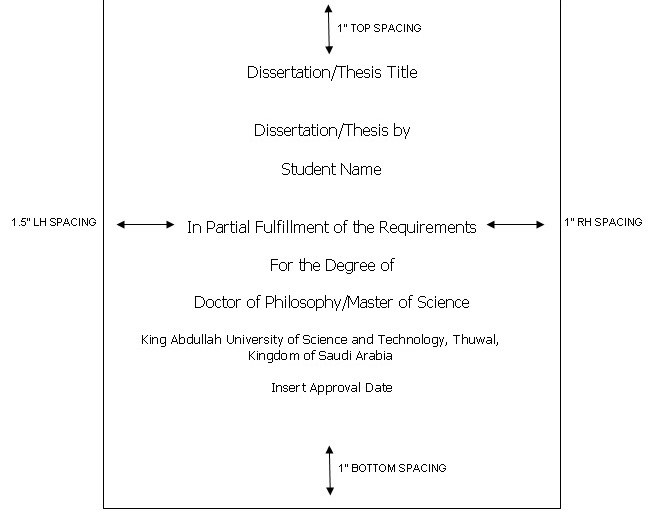
\includegraphics[scale=0.85]{Title_Page.jpg}
\caption{Sample Title Page Template \cite{guidelines}.}
\label{title_page}
\end{center}
\end{figure}

\section{Thesis Title Guidelines}

Dissertations or Theses are valuable resources for scholars that should be easily retrievable. Modern retrieval systems generally use the words in the title to locate a document. Search engines use the words in the title, and sometimes other descriptive words, to locate works. It is essential that the title be an accurate and meaningful description of the content and that obscure references be avoided. Please use these guidelines when formulating a dissertation or thesis title:

\subsection{Case}

The first and last words and all nouns, pronouns, adjectives, verbs and adverbs (if, because, as, that, etc.) are capitalized. Articles (a, an, the), coordinating conjunctions (and, but, or, for, nor), and prepositions, regardless of length, are lowercased unless they are the first or last word of the title or subtitle. Acronyms should be used sparingly throughout and they should be set in full capitals.

Examples:

\begin{itemize}
\item Solar and Wind Power
\item Engineering Technology for Developing Countries: Best Practices as Predictors of Success.
\item A Comparison of Scientific Methodologies for Determining Achievement in Graduate School Research.

\end{itemize}

\subsection{Hyphenation}

Consult a dictionary as to whether a word is hyphenated. In general words beginning with prefixes co, non, post, or re are not hyphenated unless there is a possibility of confusion (co-op, post-master's) or the root word begins with a capital letter (post-Renaissance). Hyphenate words beginning with the prefix self. Hyphenate compounds used as adjectives (decision-making) but not as nouns (decision maker). Part-time is always hyphenated. When more than one prefix is joined to a base word, hyphenate the prefixes standing alone (micro - and macroeconomics). Do not hyphenate fundraising, freelance, yearlong or health care.

Example:

\begin{itemize}
\item Important Advances in Nonlinear Equations in the Twentieth Century (Instead of: Important Advances in Non-linear Equations in the 20th Century)

\end{itemize}

\subsection{Spelling and Grammar}

Dissertation or thesis titles should be spell-checked and dictionary spelling of words should be used.  Use "and" rather than "\&", and spell out names of centuries and other numbers.

Example:

\begin{itemize}
\item The Twentieth Century Scientific Method in Perspective.

\end{itemize}

\subsection{Special Characters}

No special characters should appear in the dissertation or thesis title.  Terms or phrases that include special characters should instead be written out.  When possible, use word substitutes for formulas, symbols, superscripts, Greek letters, etc., which do not appear on most computer keyboards and would render your title unsearchable.

Example:

\begin{itemize}
\item Hybrid MPI-CUDA Strategies for GPU-based Computational Science and
Engineering Applications on Millions of Cores (instead of Hybrid
MPI-CUDA Strategies for GPU-based CS\&E Applications on 10**6 Cores).

\end{itemize}

\subsection{Italicization}

Italics should only be used in dissertation or thesis titles when referring to the title of a published work, foreign language words, gene names, scientific names as appropriate or other words that are usually italicized.

Example:

\begin{itemize}
\item Techniques in Pseudomonas Aeruginosa Biofilus Biology

\end{itemize}

\subsection{Apostrophes}

Do not use to form plurals (it should be 1980s, not 1980's) unless it would be confusing without (thus A's B's, not As and Bs; p's, not ps).  Possessives of singular nouns ending in s are formed by adding s (e.g., Harris's cat).

\section{Signature Approvals Page}

The signature approvals page must contain original signatures verifying that the dissertation or thesis and their contents have been examined and approved by the committee members. It should only contain the signatures of the certifying members of the dissertation or thesis examination committee.

The student's name as recorded by KAUST also appears on the signature approvals page. The name should be the same as that which appears on the title page and copyrght page (if the copyright is being registered). The name of each signing committee member should be typed. No titles or degree designations should be used (no Professor, no PhD, etc.). On the signature page, the title Committee Chair or Co-Chair follows each Chair's name. The student should adjust the spacing between listed names according to how many committee members there are.  There is no required order for the names of the committee members except the name of the Chair (or Co-Chairs), which appears as the last names(s) on the page. Signatures should be in black ink. The date at the bottom of the page is the year in which the degree is awarded and is the same as the year on the title page.

The signature page is always page 2 of the manuscript, and is the first page on which a number appears. Every page after this page is numbered.

The \underline{\textbf{signature approvals page is a mandatory part}} of the dissertation or thesis submission process.

\section{Sample Copyright Page}

This is an example of the copyright page, which is optional but must follow the signature approvals page and, if included, would be numbered page 3 at the top.  

If you wish to give users the right to copy and distribute your work provided they give you credit, such as via a Creative Commons license (http://creativecommons.org/\\choose/), you may insert the relevant notice following your copyright notice (e.g., "This work is licensed under a Creative Commons Attribution 3.0 Unreported License (http://creativecommons.org/licenses/by/3.0/)."

NOTE: The year on the copyright page must be the same as the year that the author received his/her dissertation or thesis approval.

Use the same margins as the title page. The copyright page template can be seen in figure \ref{copyright_page}.

\begin{figure}[H]
\begin{center}
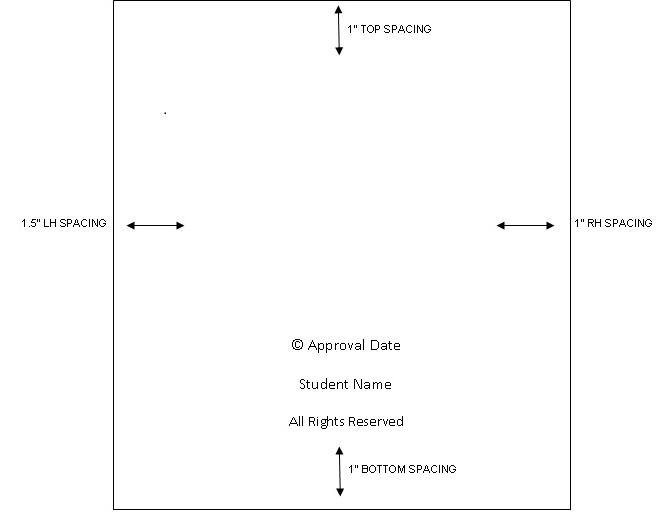
\includegraphics[scale=0.85]{Copyright_Page.jpg}
\caption{Copyright Page Template \cite{guidelines}.}
\label{copyright_page}
\end{center}
\end{figure}

% Copyright 2010 Imran Shafique Ansari
% Contact Email: imran.ansari@kaust.edu.sa
% Contact Number: +966 59 897 1005


% Chapter 3 File

\chapter{Editings}
\label{chapter3}

\section{Language and Length}

The dissertation or thesis must be written in English.  There is no specific requirement for the page length of a dissertation or thesis.  Work closely with your Thesis Advisor to plan, outline, write, and revise the text of the document. Writing a thesis or dissertation is an iterative process of written revisions.

\section{Table of Contents}

As a page heading, use "TABLE OF CONTENTS" all in capital letters, centered on the page. The format of the table should conform to the pagination guidelines and accurately reflect the outline and organization of the manuscript. List the sections/chapters of the body of the dissertation or thesis; also list preliminary sections starting with the signature approvals page and supplementary sections such as References and Appendices. The table of contents may be single-spaced.

\section{Proofreading and Editing}

All manuscripts should be proofread before being submitted to the Thesis Advisor. The consistency and accuracy of the spelling, punctuation, capitalization, abbreviations, and word divisions are primarily the responsibility of the dissertation or thesis writer, who should consult a dictionary and a manual of style for correct usage. Students need to adopt a consistent style throughout the dissertation or thesis. Students are especially urged to use the "spell-check" feature of the computer software being used and to proofread the manuscript carefully, or to enlist the help of a friend or professional proofreader. The Thesis Advisor will return to the student for correction and resubmission any dissertation or thesis that has not been carefully proofread. Students should also allow at least two weeks for proofreading before the final presentation/examination is scheduled.

Similarly, the dissertation or thesis writer is fully responsible for editing the style and grammar of the manuscript and for seeking support and assistance when necessary.

\section{Reproduction}

The following guidelines should be adhered to:

\begin{itemize}
\item	Print the final copies of your manuscript on high-quality archival bond paper, minimum 20-pound weight, and 8.5 by 11 inches in size. 
\item	All textual material should be double-spaced, but long quotations and footnotes may be single-spaced and indented. Follow the style manual chosen by your Thesis Advisor or department because these guidelines vary. 
\item	The typeface, including headers, page numbers, and footnotes - must be produced with the same font or typeface throughout the document. Exceptions are made only for tables and figures. Suggestions: TIMES NEW ROMAN 12; ARIAL 12; BOOKMAN 12; GARAMOND 12; CAMBRIA 12.

\end{itemize}

\section{Footnotes and Endnotes}

Footnotes may be single-spaced in a 10-point size but must be in the same font as the rest of the text. Footnotes should be numbered with superscripted Arabic numbers. Numbering must be continuous throughout the document. Users of LaTeX may use CMR 12 font or any font that meets the above specifications. The print should be letter quality with dark black characters that are consistently clear and dense.

\section{Justification}

Left-aligned, ragged right margins are preferred. Use justified margins only if the computer does this well, i.e., does not separate punctuation from characters or leave large gaps in the text.

\section{Margin}

\begin{itemize}
\item Left margin - 1.5 inches
\item Right margin - 1 inch
\item Top and bottom	- 1 inch

\end{itemize}

Exact margins are absolutely essential so that the thesis can be digitized in its entirety for interlibrary loan. The same width margins must apply to all pages, including those containing graphs, tables, and other illustrative materials.

\section{Pagination}

All pages except the title page must be numbered at least 0.75" from the top of the page. Begin the numbering with Arabic numbers on the top of the page following the title page. Use continuous Arabic numbers beginning with the signature approvals page (page 2) and continue with every sheet that follows, whether it is text, figures, explanation for figures or photos, tables, maps, appendices, etc., numbering pages to the end. Page numbers must be within the margins at the top of each page.

Each chapter must be numbered separately, using consecutive Roman numerals to distinguish the individual chapters throughout the dissertation or thesis. Chapters within the text begin on new pages. There should be no page breaks between sections or before tables or figures, unless they occur naturally.

Paginate the parts of the dissertation or thesis in the order as shown in table \ref{table}:

\begin{table}
\centering\caption{Parts Pagination \cite{guidelines}} \label{table}
\begin{tabular}{|c|l|c|}\hline
\textbf{S.~No.} & \textbf{Page Style/Type} & \textbf{Page Numbering} \\\hline\hline
 1. & Title Page                      & (not numbered)\\ \hline
 2. & Signature Approvals Page        & 2\\ \hline
 3. & Copyright Page (if applicable)  & 3\\ \hline
 4. & Abstract                        & 4\\ \hline
 5. & Acknowledgments (Optional)      & 5\\ \hline
 6. & Table of Contents               & 6\\ \hline
 7. & List of Abbreviations           & 7\\ \hline
 8. & List of Symbols (Optional)      & 8\\ \hline
 9. & List of Illustrations           & 9\\ \hline
10. & List of Tables                  & 10\\ \hline
11. & Main text of thesis,            & \\
    & including any Introduction or Summary. & \\ \hline
12. & Material to follow text,        & \\
    & such as references, appendices, & \\
    & and fold-in maps. However,      & \\
    & such material may be included   & \\
    & at the end of each chapter,     & \\
    & making each chapter a complete  & \\
    & and self-contained paper,       & \\
    & nonetheless with pagination in  & \\
    & sequence with the remainder of the thesis. & \\ \hline
\end{tabular}
\end{table}

\section{Equations, Formulas, Sub/Superscripts}

All equations and formulas should be typeset. When a computer or word processor cannot make a symbol, insertions by hand are acceptable. All subscripts and superscripts must be large enough to be clearly read.

\section{Charts, Graphs, Tables, Photographs, and Oversized Maps}

Illustrations must be of equally high quality in the "final" copies submitted to the Offices of the Provost, Associate Provost of Graduate Affairs and to the library. For the digital copy of your work submitted to the library, illustrations must be inserted as an image at the appropriate place within the thesis or dissertation.

Please keep in mind:

\begin{itemize}
\item Labels or symbols rather than colors should identify lines on a graph.
\item	Shaded areas---such as countries on a map---will have better contrast if cross-hatching is used instead of color. 
\item	Photographs should be professional-quality black and white or color.  Most photographs will reproduce acceptably on positive microfilm or microfiche but will lack clarity on photocopies made from the microfilm.  If color copies are necessary, all final copies of the dissertation or thesis should include the color photographs.  
\item	Charts, graphs, and maps that are larger than the standard 8.5" x 11" page size may be used in your manuscripts.  They should be carefully folded into the manuscript or rolled up and placed in a mailing tube.

\end{itemize}

\section{Plagiarism Checking}

All students are required to have their manuscripts checked by Skills Lab personnel using the 'Turn It In' plagiarism software. The resulting originality reports will be submitted to the office of the Associate Provost of Graduate Affairs for review and approval.  Copies of the approved reports will be forwarded to the Graduate Program Coordinators and to the library.  This is a mandatory part of the graduation process.

\section{Use of Copyrighted Material}

As the author of the dissertation or thesis manuscript, you will be asked to certify that any previously copyrighted material used in your work, beyond "fair use," is with written permission of the copyright owner, and that KAUST will not be held responsible for any damages which may arise from copyright violations.  When depositing your work in the KAUST digital archive, you will be required to warrant that you have obtained all necessary rights. (Please see 'sample permission letter' on page 19 of \cite{guidelines}).

In most cases no problem will arise if your evaluation of the circumstances suggests the use is fair. Your evaluation should weigh four factors:

\begin{itemize}
\item Purpose and character: Because your use is for non-profit educational purposes, this is a factor favoring fair use. But if you are to derive payment from use of the dissertation or thesis, this would weigh against fair use.
\item Nature of copyrighted work: Is the work fact based, published, or out-of-print? These factors weigh in favor of fair use.
\item Amount used:  Using a small portion of a whole work would weigh toward fairness.
\item Market effect: A use is more likely to be fair if it does not harm the potential market for or value of the copyrighted work. But if it does, this could weigh more heavily against fair use than the other factors.
\end{itemize}

Consider each of these factors, but all of them do not have to be favorable to make your use a fair one. When the factors in the aggregate weigh toward fairness, your use is better justified. When the factors tip the scales in the other direction, your need to obtain permission from the copyright holder increases. Don't worry that the answer isn't crystal clear. Just decide whether the factors weigh enough toward fairness so that you are comfortable not seeking permission.

KAUST Library offers links to more information on copyright and permissions on their theses and dissertations webpages at http://libguides.kaust.edu.sa/theses.

\section{Use of Published Material}

Published articles of which the candidate is author or joint author may be included as part of the dissertation or thesis, with due regard to copyright regulations (see previous section). For the "original copy" of the manuscript, such printed pages must follow the same requirements as outlined in this guide, maintaining margins, type size (at least 12 point), page number sequencing, etc.

\section{Some Common Errors}

\begin{itemize}
\item Unnumbered pages, especially those containing figures or captions to figures.
\item	Names of authors spelled differently in the text and in the bibliography; reference numbers or dates in the text that do not agree with the bibliography.
\item	Inconsistent presentation of bibliographic information.
\item	Incorrect punctuation of abbreviations.  The Latin abbreviation for "and others" contains only one period "et al."  The abbreviations "i.e." and "e.g." are punctuated with two periods and set off by commas from the sentences in which they appear, unless a specific style manual required by your advisor or department suggests otherwise, as some do.
\item	Inconsistent hyphenation of compound words.
\item	Inconsistent capitalization of proper nouns used as adjectives.
\item	Reversed punctuation of quotations.  Periods and commas always precede final quotation marks, even if the quotation consists of a single letter unless your text follows the quotation in the sentence.

\end{itemize}

\section{Some Common Formatting Errors}

\begin{itemize}
\item The page size should be 8.5  x 11 inches (regular US letter size)
\item	Incorrectly sized margins - the left margin should be 1.5" inches and all other margins 1 inch.
\item	All pages should be numbered consecutively (except for the title page) and the numbers should be correctly placed on the page - at least 0.75 inches from the top of the page.  
\item Pages should be ordered properly, with the title page first, followed by the signature approvals, copyright, and then the abstract pages. Check for missing pages.
\item	The abstract should be 350 words or less.
\item	The title page should include the correct date - the date should be the month and year you will receive the degree, for example December 2011.
\item	The correct number of copies should be submitted.
\item	You must have permission to use previously published material.

\end{itemize}

% Copyright 2010 Imran Shafique Ansari
% Contact Email: imran.ansari@kaust.edu.sa
% Contact Number: +966 59 897 1005


% Chapter 4 File

\chapter{Miscellaneous}
\label{chapter4}

\section{Instructions for Permission Letters}

\begin{itemize}
\item Include your return address, telephone number and email address, and date the top of the letter. 
\item	Confirm the exact name and address of the addressee. Call the person to confirm the copyright ownership.
\item	State clearly the name of your university and your thesis title. 
\item	Describe precisely the proposed use of the copyrighted material. If necessary or appropriate attach a copy of the quotations, diagrams, pictures, and other materials. If the proposed use is extensive, such as the general use of an archival or manuscript collection, describe it in broad and sweeping terms. Your objectives are to eliminate any ambiguities and to be sure the permission encompasses the full scope of your needs. 
\item	The sample signature form at the end of the sample letter is appropriate when an individual grants the permission. When a company, such as a publishing house, is granting permission, use the following signature form.

\end{itemize}

\section{Some important checks}

\begin{itemize}
\item Appendices can be referred/cited as Appendix \ref{appendixB}.
\item Equations can be referred using 'eqref' command.
\item Bibliography can have different types of references such as conference proceedings \cite{key1}, journal articles \cite{key2}, books \cite{key3}, miscellaneous references including web links etc. \cite{key4}, and theses/dissertations \cite{key5} among others.

\end{itemize}

% Copyright 2010 Imran Shafique Ansari
% Contact Email: imran.ansari@kaust.edu.sa
% Contact Number: +966 59 897 1005

\chapter{Creating the List of Abbreviations and List of Symbols}\label{chapter5}
\lstset{basicstyle={\ttfamily,\small}, frame=lines}

\section{Introduction}
The most versatile package to create the \gls{loa} and \gls{los} is currently the \texttt{glossaries} package. With the \texttt{glossaries} package, one can create those and even more lists all in the same document. Every list is sorted alphabetically and can even have the page numbers where the entries appear (if that's desired) just like an ``Index of terms'' list. 

In the following there is a description on how to use the \texttt{glossaries} package. The material is taken from the documentation of the package and some other examples that can be found online.


\section{How to use the \texttt{glossaries} package}\label{sec:howto}
The \texttt{glossaries} package works more or less like the \texttt{Makeindex}. In fact one needs to use the \texttt{makeindex} command to actually create the lists (see \S\ref{sec:printlists}). The main difference is that when creating an index, one only has to define the index terms in the text, using an \texttt{\textbackslash index\{}\textit{term}\texttt{\}} command. On the other hand, in order to create the \gls{loa} and \gls{los} one needs to define those entries and use a \texttt{\textbackslash gls\{}\textit{term}\texttt{\}} or similar command to reference them in the text. 

The definition of those entries must be in the preamble right after the definition of all the lists and the \texttt{\textbackslash makeglossaries} command. It is probably a good idea to have them in a separate file, which you include (as is done in the example \texttt{Thesis.tex} with the \texttt{\textbackslash include\{Lists\}} command). 

The general format for entries is\\
\texttt{\textbackslash newglossaryentry\{}\textit{label}\texttt{\}\{}\textit{definition}\texttt{\}}\\
The first argument (\textit{label}) is a label that \emph{uniquely} identifies this entry. The second argument (\textit{definition}) is a comma-separated list of \texttt{key=}\textit{value} pairs. For example
\begin{lstlisting}
\newglossaryentry{datacomp}{name=data compression, description=
the  process of encoding information using less bits than the 
original representation uses}
\end{lstlisting}
In this example there are two keys, namely the \texttt{name} and the \texttt{description}. The key \texttt{name} has the value ``data compression'' and the key \texttt{description} has the value ``the process... uses''. The \texttt{glossaries} package understands that a key value ends when it encounters a comma and treats the next word as a key. The value of the key \texttt{name} is what will appear in the text when referenced by a \texttt{\textbackslash gls\{datacomp\}} command. The value of the key \texttt{description} is what will appear in the default Glossary (or any other) list.


\subsection{Glossary entries}
\lstset{basicstyle={\ttfamily,\small}, frame=lines}
Some more examples of glossary or symbols entries are given below.
\begin{lstlisting}
\newglossaryentry{elite}{name={\'e}lite, description=select
group or class, sort=elite}
\end{lstlisting}

In this example notice the use of \texttt{\{\textbackslash'e\}} notation to produce the accented letter {\'e}. Because \texttt{makeindex} will not know how to sort this alphabetically (\texttt{makeindex} is hardcoded for english), it is a good idea to use the key \texttt{sort} to specify how we want this entry to be sorted. In this example the entry ``\'elite'' will be treated as if it were ``elite''.
\begin{lstlisting}
\newglossaryentry{pi}{name={\ensuremath{\pi}}, sort=pi, 
description={ratio of circumference of circle to its diameter}}
\end{lstlisting}

In this example the entry is $\pi$. Notice the \texttt{\textbackslash ensuremath\{\}} command which makes sure that the term \texttt{\textbackslash pi} is indeed in math mode (if it isn't then it prepends and appends the \$ sign) so that LaTeX doesn't throw an error. Also notice that the curly brackets enclosing the \texttt{description} value are not mandatory here but they \emph{should} be used if the description value contains a comma. Otherwise the \texttt{glossaries} package will understand that the comma denotes the end of the value and treat the following word as a key. 
\begin{lstlisting}
\newglossaryentry{ohm}{name=ohm, symbol={\ensuremath{\Omega}},
description=unit of electrical resistance}
\end{lstlisting}

This example defines an entry for both the Glossary list (due to the key \texttt{name}) and the \gls{los} (due to the key \texttt{symbol}).

\subsection{Abbreviation (Acronym) entries}
Acronym entries can be defined using \texttt{\textbackslash newglossaryentry} command but there is also a handy shortcut, namely the \texttt{\textbackslash newacronym} command. For example
\begin{lstlisting}
\newglossaryentry{led}{name=LED, description={light-emitting 
diode}, first{light-emitting diode (LED)}
\end{lstlisting}
is equivalent to the much shorter 
\begin{lstlisting}
\newacronym{led}{LED}{light-emitting diode}
\end{lstlisting}
Note that the first time the entry \texttt{led} is found, the \texttt{glossaries} package will print the description followed by the acronym in parentheses i.e.\ ``light-emitting diode (LED)'' (this is actually what the key \texttt{first} is for in the \texttt{\textbackslash newglossaryentry} command).

Also calling \texttt{\textbackslash acrlong\{led\}} will produce ``Light-Emitting Diode'' (i.e.\ the \emph{long} version of the entry ---the description) while \texttt{\textbackslash acrshort\{led\}} will produce ``LED'' (i.e.\ the \emph{short} version of the entry ---the acronym).

\subsection{Symbols entries}
Entries for the List of Symbols follow the exactly same rule as the glossary entries, with the addition of \texttt{type=symbols} in the definition part of the entry. For example
\begin{lstlisting}
\newglossaryentry{pi}{type=symbols, name={\ensuremath{\pi}},
description={ratio of circumference of circle to its diameter}, 
sort=pi}
\end{lstlisting}
If the key \texttt{type} is omitted, the main glossary (i.e.\ the Glossary) is assumed.

\section{Referencing the entries in the text}
In order to reference the entry in the text one just has to write \texttt{\textbackslash gls\{}\textit{label}\texttt{\}}. For example for the glossary entry \texttt{datacomp} defined in \S\ref{sec:howto}, one just has to write \texttt{\textbackslash gls\{datacomp\}}
which will produce the value of the key \texttt{name}, i.e.\ ``data compression''. Note that 
\begin{itemize}
   \item \texttt{\textbackslash Gls\{datacomp\}} will produce ``Data compression'' (i.e.\ the first is capital), 
   \item \texttt{\textbackslash GLS\{datacomp\}} will produce ``DATA COMPRESSION'' (i.e.\ all capital), 
   \item \texttt{\textbackslash glspl\{datacomp\}} will produce ``Data compressions'' (i.e.\ plural),
   \item \texttt{\textbackslash Glspl\{datacomp\}} will produce ``Data compressions'' and
   \item \texttt{\textbackslash GLSpl\{datacomp\}} will produce ``DATA COMPRESSIONS''.
\end{itemize}
The plural form is formed by just appending an ``s''. If the plural form of an entry is different, one just has to define it in the definition part using the key \texttt{plural}. For example
\begin{lstlisting}
\newglossaryentry{bus}{name=data bus, description=a subsystem 
that transfers data between computer components, plural=buses}
\end{lstlisting}

There are quite a few more keys in the documentation of the package that allow even more flexibility.


\section{Printing the lists}\label{sec:printlists}
The following piece of code is already in the \texttt{Thesis.tex} file. Here is an explanation of what each line does, in case something need to be modified.

\begin{lstlisting}[numbers=left,numberstyle=\footnotesize]
\printglossary[type=\acronymtype,style=long, title=List of 
               Abbreviations, toctitle=List of Abbreviations, 
               nonumberlist=true] 

\printglossary[type=symbols,style=long]   

\printglossary[style=altlist, toctitle=Glossary, nonumberlist=true] 
\end{lstlisting}

Lines 1-2 should appear where you want the List of Abbreviations to appear. They will print the entries and show them in the document's \gls{toc}. Notice that I had to change the default title ``List of Acronyms'' to ``List of Abbreviations'' for both the chapter title and the \gls{toc} entry.

Line 4 should appear where you want the List of Symbols to appear. It will print the symbols entries and show them in the document's \gls{toc}.

Lines 6-8 should appear if you would like to have a Glossary (optional). They will print the Glossary entries and show an entry ``Glossary'' in the document's \gls{toc}. The \texttt{nonumberlist=true} suppresses the page numbers in the list.

In order to actually see the lists in your document, you need to run LaTeX once and then run the following commands in the command line (they can also be found in the preamble of the \texttt{Thesis.tex} as comments):
\begin{lstlisting}
makeindex -s Thesis.ist -t Thesis.alg -o Thesis.acr Thesis.acn
makeindex -s Thesis.ist -t Thesis.slg -o Thesis.syi Thesis.sbl
makeindex -s Thesis.ist -t Thesis.glg -o Thesis.gls Thesis.glo
\end{lstlisting}
If your main input file is not \texttt{Thesis.tex}, then replace all the occurences of \texttt{Thesis} with that filename. Then run LaTeX once again.

Sometimes (depending on the entries) this procedure has to be repeated once more.

\section{Test section}
In this section there is some text,used to show how the \texttt{glossaries} package. See the source file of this chapter and of the Introduction for the exact usage. 

\subsection{General information}
Our network uses \gls{AD}. By using \gls{AD} with \gls{M$} bases clients that
have been installed using a \gls{glos:RespF} from \gls{CD}, we can expect a 
high level of standardization.

\subsection{Some Greek symbols}
If you multiply a rational with \gls{symb:Pi} you always get an irrational result, because 
\gls{symb:Pi} itself is irrational. As a matter of fact, so are \gls{symb:Phi} 
and \gls{symb:Lambda}, too.




% Conclusion File

\chapter{Concluding Remarks}

\section{Summary}

The author must provide an overall summary and discussion of the significance of the work. If the dissertation or thesis consists of relatively independent chapters, a unifying summary should be included at the end or beginning of the dissertation or thesis. Such a summary will be significantly more expansive than the abstract.

\section{Bibliography (or References or Works Cited)}

As a page heading, use "BIBLIOGRAPHY" (or "REFERENCES" or "WORKS CITED") all in capital letters centered on the page. Always start a new page. Bibliographies may be single-spaced within each entry but must include 24 points of space between entries. It is recommended that you follow the standard citation format used by a major journal in your academic field and that the style be consistent throughout the dissertation or thesis.

\section{References}

The precise form of a bibliography or reference section can conform to the style current in the thesis or dissertation writer's discipline, but this form must be employed consistently throughout the thesis. All material already published must be reformatted into the guidelines specified here and pagination and bibliographic style should be consistent with the remainder of the document. For MS Word users, the EndNote citation management software can be utilized as a referencing tool. It is available for download by KAUST students via the KAUST Library website.  

A variety of helpful guides to bibliographic style in various fields are available from KAUST Library, including:

\begin{itemize}
\item\underline{The ACS Style Guide: Effective Communication of Scientific Information.}\\ \underline{Anne M. Coghill and Lorrin R. Garson, editors.} 3rd ed.  Washington, D.C.: American Chemical Society, 2006.
\item\underline{The Chicago Manual of Style.} 16th ed. Chicago, IL: University of Chicago Press, 2010.
\item\underline{A Manual for Writers of Research Papers, Theses, and Dissertations. Kate L.}\\ \underline{Turabian.} 7th ed. / Chicago, IL: University of Chicago Press, 2007.
\item\underline{MLA Style Manual and Guide to Scholarly Publishing.} 3rd ed. New York: Modern Language Association of America, 2008.
\item\underline{Scientific Style and Format: The CSE Manual for Authors, Editors, and}\\ \underline{Publishers.} 7th ed.  Council of Science Editors, 2006.
\item\underline{United States Government Printing Office Style Manual.} 30th ed. Washington, D.C.: U.S.G.P.O., 2008. (Also online: http://www.gpoaccess.gov/stylemanual/\\browse.html)
\item In addition, many technical journals publish appropriate style rules.
\item For more resources on scholarly writing, visit the Library's theses and dissertations webpages at http://libguides.kaust.edu.sa/theses.

\end{itemize}

\section{Submission of Thesis}

As soon as you have received approval of your thesis or dissertation, you must submit the full final approved document to the KAUST digital archive in the library. You may not submit a draft or partial document. Please follow these submission instructions:

Convert your file to a PDF. Please name the PDF with your first and last name (e.g., RashedAlzahraniThesis.pdf). Be sure this is the full, final copy that your committee has approved. Submit the PDF according to instructions on the library's theses and dissertations webpages at http://libguides.kaust.edu.sa/theses.

The submission of dissertations or theses to the library is determined by the library's policies and guidelines. For more information on the online status of your document or policies and guidelines please contact library personnel.

\section{Future Research Work}

The work presented in this thesis can be extended in the following directions.

List of your planned future work goes here.

% Copyright 2010 Imran Shafique Ansari
% Contact Email: imran.ansari@kaust.edu.sa
% Contact Number: +966 59 897 1005


\appendix

\begin{center}
\vspace*{\fill}
\thispagestyle{empty} 
{\bf\Huge\centering{APPENDICES}}
\addcontentsline{toc}{chapter}{Appendices}
\vspace*{\fill}
\end{center}


% Appendix A File

\chapter{Appendix A Title}
\label{appendixA}

Detailed experimental procedures, data tables, computer programs, etc. may be placed in appendices. This may be particularly appropriate if the dissertation or thesis includes several published papers.

% Copyright 2010 Imran Shafique Ansari
% Contact Email: imran.ansari@kaust.edu.sa
% Contact Number: +966 59 897 1005



% Appendix B File

\chapter{Appendix B Title}
\label{appendixB}

Your content goes here.

% Copyright 2010 Imran Shafique Ansari
% Contact Email: imran.ansari@kaust.edu.sa
% Contact Number: +966 59 897 1005



% Appendix for Papers

\chapter{Papers Submitted and Under Preparation}

$\bullet$ Author 1 Name, Author 2 Name, and Author 3 Name, {``Article Title"}, \emph{Submitted to Conference/Journal Name}, further attributes.
\\
$\bullet$ Author 1 Name, Author 2 Name, and Author 3 Name, {``Article Title"}, \emph{Submitted to Conference/Journal Name}, Mon. Year.

% Copyright 2010 Imran Shafique Ansari
% Contact Email: imran.ansari@kaust.edu.sa
% Contact Number: +966 59 897 1005


\renewcommand*\bibname{Bibliography/References} 
\addcontentsline{toc}{chapter}{References}
\bibliographystyle{IEEEtran}
\bibliography{References}


\end{document}

% Copyright 2010 Imran Shafique Ansari
% Contact Email: imran.ansari@kaust.edu.sa
% Contact Number: +966 59 897 1005
